% !TEX root = cha-soa.tex
\documentclass[../../main.tex]{subfiles}

\begin{document}

\section{Graph-Based Visualizations}
\label{sec:graph-based_visualization}
Software systems can naturally be represented as graphs \citebibliography{DiBa1998a}, where software entities (such as classes or packages) are represented as nodes, and their relationships (such as dependencies or method calls) are represented as edges. To enhance graphs readability, various layout strategies have been proposed.

\subsection{Force-Directed Layout} Fruchterman and Reingold~\citebibliography{Fruc1991a} introduced a widely used layout algorithm based on a physical analogy. The algorithm is designed for undirected graphs and aims to distribute nodes evenly on the frame while keeping connected nodes close and reducing edge crossings. Nodes act as particles that repel each other, while edges act as springs that attract connected nodes. Starting from an initial node placement (that can be random), these forces move the nodes until the system reaches a stable state. The resulting layout should follow two main principles: connected nodes should be placed near each other, but nodes should not be placed too close to each other.
     
\subsection{Orthogonal Layouts} Tamassia~\citebibliography{Tama1987a} introduced an approach for orthogonal graph drawing where edges follow horizontal and vertical lines on a rectilinear grid. The method aims to minimize the total number of bends while preserving the original planar structure of the graph. To achieve this, the problem is transformed into a minimum-cost flow problem, where the cost of the flow corresponds to the number of bends. The algorithm can then compute an orthogonal representation with the minimum number of bends in $O(n^2 \log n)$ time. This approach is useful for automatic layout of graph-based diagrams, where horizontal and vertical segments can provide a clear and structured representation.

\subsection{Edge Bundling} Holten~\citebibliography{Holt2006a} introduced hierarchical edge bundling to reduce visual clutter in compound graphs. Instead of drawing relationships as straight lines, edges are curved along paths between nodes. This technique groups edges into bundles, clarifying connections between groups. Bundling strength is adjustable: lower values ($\beta = 0$) make individual connections easier to follow, while higher values ($\beta = 1$) highlight relationships between groups of nodes. An example is shown in \figref{fig:edge_bundling}.

\begin{figure}[ht]  
    \centering 
    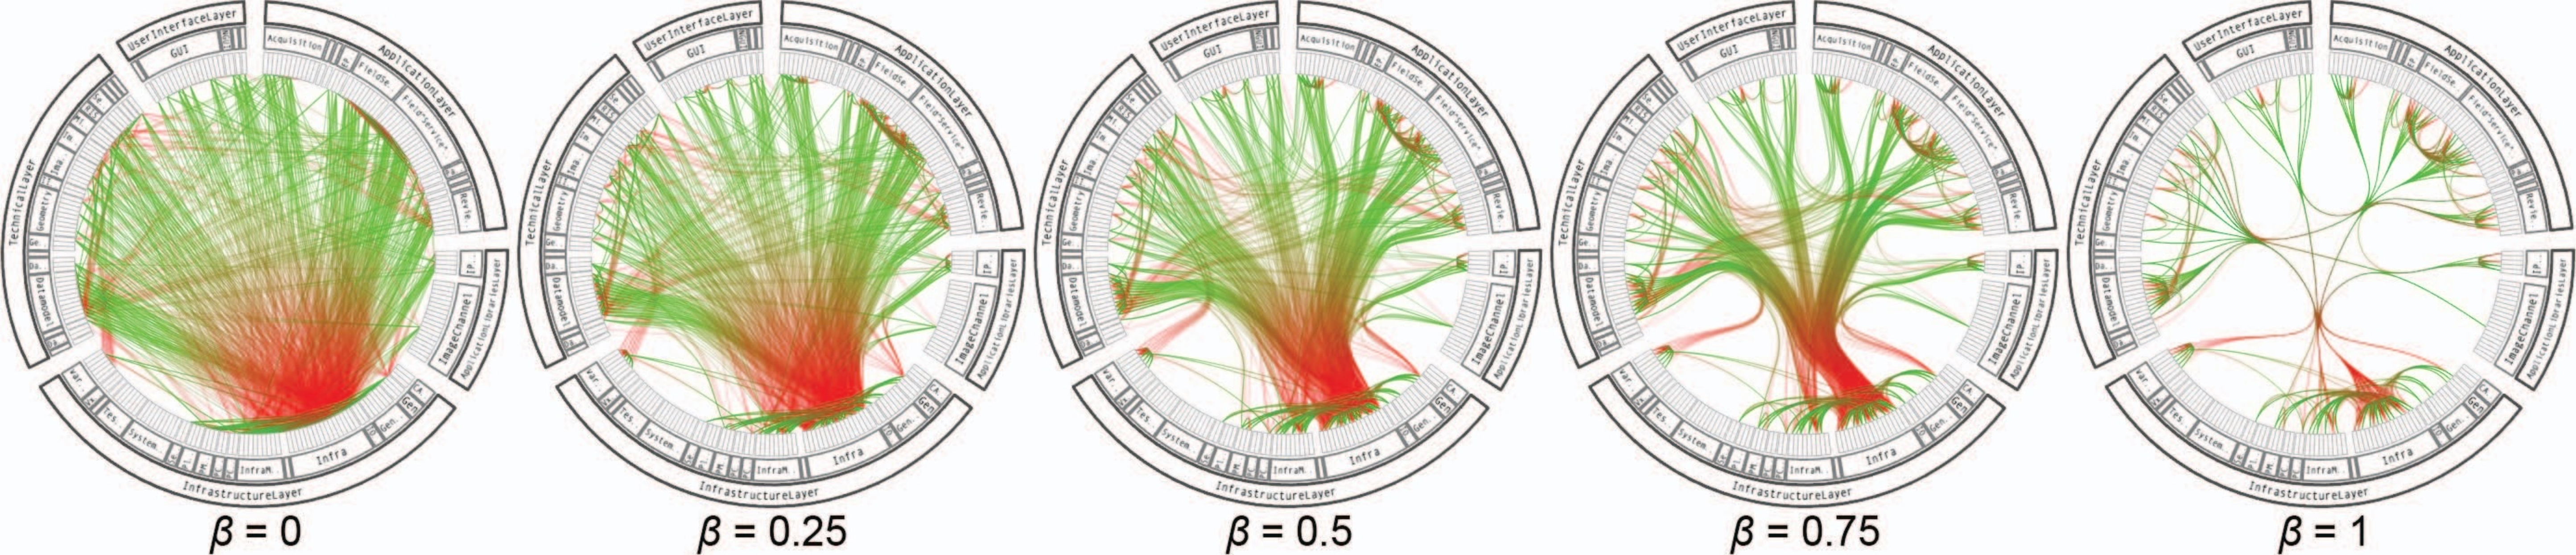
\includegraphics[width=0.85\linewidth]{figures/soa/edge_bundling} 
    \caption[Example of Edge Bundling.]{Example of Edge Bundling~\citebibliography{Holt2006a}.}
    \label{fig:edge_bundling}
\end{figure}

\end{document}